\documentclass[a4paper,11pt]{exam}
\usepackage[utf8]{inputenc}
%\usepackage{lipsum}

\date{October 26, 2018}%\today}
\title{RE355 - Introduction to Cloud Networking \\
Lab session 1: A gentle introduction to Docker}
\author{Dr. Inti González Herrera \and Dr. Nicolas Herbaut \and Pr. Laurent Réveillère \and M. Simon Da Silva \and M. Mathias Lacaud}

%\usepackage{fancyhdr}
\usepackage{listings}
\usepackage{graphicx}
\usepackage{hyperref}

%\pagestyle{fancy}
%\fancyhf{}
\rhead{Bordeaux INP: ENSEIRB-MATMECA}
\lhead{RE355 - Introduction to Cloud Networking}


\lstset{language=sh,basicstyle=\ttfamily,columns=fullflexible}
\begin{document}
		
\maketitle

\section{Introduction}

\subsection{Docker and the wonderful world of containers}

Cf. document \textbf{Docker Presentation} on Moodle.

\subsection{Discovering docker}

\subsubsection{Installation}

Follow the \textbf{Setup instructions} on Moodle to setup your machines.
Do not hesitate to ask your teaching assistant in case of trouble!

Docker should now be installed on your machine. Check that everything works with

\begin{lstlisting}[frame=single,language={sh}]  % Start your code-block

$ docker run hello-world
\end{lstlisting}
\begin{center}
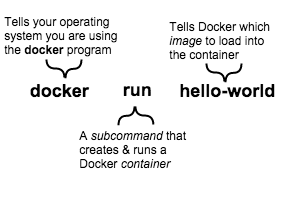
\includegraphics[width=8cm]{container_explainer.png}	
\end{center}


\subsection{Basic command line} \label{sssec:commandline}

This is a quick description of the docker command line. If you don't know docker, go through these explanations. You will use them in the rest of the lab.

\subsubsection*{Downloading a pre-built image}

We created a custom ubuntu image, ubuntu\_re355, which is the base ubuntu image with many network and system utilities installed to save you some time!

\begin{lstlisting}[frame=single,language={sh}]  % Start your code-block

$ docker pull mlacaud/ubuntu_re355
\end{lstlisting}

\subsubsection*{Running an interactive shell}
\begin{lstlisting}[frame=single,language={sh}]  % Start your code-block

$ docker run -i -t mlacaud/ubuntu_re355 /bin/bash       
\end{lstlisting}

The -i flag starts an interactive container. The -t flag creates a pseudo-TTY that attaches stdin and stdout.

To detach the tty without exiting the shell, use the escape sequence Ctrl-p + Ctrl-q. The container will continue to exist in a stopped state once exited. To list all containers, stopped and running, use the docker ps -a command.

\subsubsection*{Selecting the name of the containers}
By default, containers have an ID (hex string) and an auto-generated name. You can force a particular name for convenience.
\begin{lstlisting}[frame=single,language={sh}]  
$ docker run --name containerX -i -t mlacaud/ubuntu_re355 /bin/bash       
\end{lstlisting}



\subsubsection*{Starting a long-running worker process}
\begin{lstlisting}[frame=single,language={sh}]  % Start your code-block

# Start a very useful long-running process
$ JOB=$(docker run -d mlacaud/ubuntu_re355 /bin/sh -c "while true;\
 do echo Hello world; sleep 1; done")

# Collect the output of the job so far
$ docker logs $JOB

# Kill the job
$ docker kill $JOB
\end{lstlisting}

\subsubsection*{Listing containers}

\begin{lstlisting}[frame=single,language={sh}]
$ docker ps # Lists only running containers
$ docker ps -a # Lists all containers
\end{lstlisting}

\subsubsection*{Controlling containers}
\begin{lstlisting}[frame=single,language={sh}]
# Start a new container
$ JOB=$(docker run -d mlacaud/ubuntu_re355 /bin/sh -c "while true; \
do echo Hello world; sleep 1; done")

# Stop the container
$ docker stop $JOB

# Start the container
$ docker start $JOB

# Restart the container
$ docker restart $JOB

# SIGKILL a container
$ docker kill $JOB

# Remove a container
$ docker stop $JOB # Container must be stopped to remove it
$ docker rm $JOB
\end{lstlisting}

\subsubsection*{Executing a command on a running container}
\begin{lstlisting}[frame=single,language={sh}]
$ docker exec -ti container_id /bin/sh
\end{lstlisting}


\subsubsection*{Attaching to a running container to the current terminal to see the outputs}
\begin{lstlisting}[frame=single,language={sh}]
$ docker attach container_id 
\end{lstlisting}

\section{Docker Containers}
Inside of a container created with Docker, applications and commands can be used in an isolated environment.

Based on section \ref{sssec:commandline}, run a custom mlacaud/ubuntu\_re355 container with an interactive shell.
\begin{questions}
	\question Environment variables
	\begin{parts} 
		\part (Global knowledge) What is the command to print the environment variables ?
		\part Print the environment variables of the computer in a new terminal. Print the environment variables of the container in the interactive shell. What can you say about the isolation of containers ?
	\end{parts}
	\question File System
	\begin{parts}
		\part (Global knowledge) Create a file \textbf{"hello.txt"} in the interactive shell of the container and indicate how you have created this file.
		\part Can you see the file using \textbf{ls} inside of the container ? Can you see the file inside of an other terminal in your computer ? Conclude.
	\end{parts}
\end{questions}

\section{Docker Networking}

\subsection{Default Bridge Network}

      
\begin{questions}

	\question Docker installed a Linux bridge docker0 in your system. 
	\begin{parts}
		\part What is its mac address? 
		\part Its IP address?
		\part The subnet it belongs to?
	\end{parts}
	
	\question Inspect the bridge with the network command

		\begin{lstlisting}[frame=single,language={sh}]
$ docker network inspect bridge
		\end{lstlisting}

	By default, containers are attached to this default bridge. Launch 2 containers named container1 and container2 with an mlacaud/ubuntu\_re355 image.
	\begin{parts}
		\part Can the two containers ping one another using their IPs?
		\part Can the two containers ping one another using their host names (you can find the container's host names within the container by typing 'echo \$HOSTNAME'?)
		\part Give the commands or tools you used to find out.	
	\end{parts}
	
	\question Stop and delete container2. Relaunch it with the following command.

		\begin{lstlisting}[frame=single,language={sh}]
$ docker run -ti --name container2 --link container1 mlacaud/ubuntu_re355
		\end{lstlisting}	
		\begin{parts}
			\part try to ping container1 from container2 using container1 hostname (eg.). What's the result?
					\begin{lstlisting}[frame=single,language={sh}]
$ container2 > ping container1
					\end{lstlisting}	
			\part what mechanism does docker use to make container2 aware of container1?
			\part what are the limitations of this technique?
		\end{parts}
		
	

\end{questions}

\subsection{Exposing ports \label{netcat}}


\begin{questions}
\question By default, you cannot access a web server running within a container because ports are not public. In this exercise you will learn how to expose them.

\textbf{Hint:} Some of the commands below don't run without modification. The problem is that the last Ubuntu image doesn't include the command \textit{nc}. To solve this issue install the package \textit{netcat-openbsd}.

\begin{parts}
\part Launch the following command and explain what it does.

\begin{lstlisting}[frame=single,language={sh}]
while true;do echo salut $HOSTNAME |nc -l 8080; done;
\end{lstlisting}	

\part 	Launch the following container image and connects on the 8080 port of the container.

\begin{lstlisting}[frame=single,language={sh}]
docker run --name container1 -d  mlacaud/ubuntu_re355 /bin/bash -c 'while true;\
do echo salut $HOSTNAME |nc -l 8080; done;'
\end{lstlisting}	

give the output of docker ps. From the host, can I establish a TCP connection to this container on port 8080? How?

\part 
Launch the following container image, 
\begin{lstlisting}[frame=single,language={sh}]
docker run -p 8080 --name container1 -d  mlacaud/ubuntu_re355 /bin/bash -c \
'while true; do echo salut $HOSTNAME |nc -l 8080; done;'
\end{lstlisting}	

give the output of docker ps. What's the difference? On which port of the localhost is the container reachable?

\part 
launch the following container image. 
\begin{lstlisting}[frame=single,language={sh}]
docker run -p 8080:8080 --name container1 -d  mlacaud/ubuntu_re355 /bin/bash -c \
'while true; do echo salut $HOSTNAME |nc -l 8080; done;'
\end{lstlisting}	

give the output of docker ps. What's the difference? On which port of the localhost is the container reachable?

\part How does docker configure port forwarding? (Hint: it is a Linux networking tool)


\end{parts}
\end{questions}

\subsection{None Network}
\begin{questions}
	\question What option of the "docker run" command allows specifying the network for the container? 
	\question Launch a container with the "none" configuration. Describe its network connectivity.
\end{questions}


\subsection{Custom Bridged Network}


It's possible to create isolated networks on which the containers will be attached.
\begin{lstlisting}[frame=single,language={sh}]
$ docker network create --driver bridge network1
\end{lstlisting}

more info on the network can be retrieved with the inspect command

\begin{lstlisting}[frame=single,language={sh}]
$docker network inspect network1
[
    {
        "Name": "network1",
        "Id": "7009786ffb94f650eb1a71395cac3b28f68bbdcb9112662b6bedb0",
        "Scope": "local",
        "Driver": "bridge",
        "IPAM": {
            "Driver": "default",
            "Config": [
                {}
            ]
        },
        "Containers": {},
        "Options": {}
    }
]
\end{lstlisting}

\begin{questions}
	\question create 2 new bridged networks named network1 and network2. Create container1 on network1 and container2 on network2. Give the commands.
	\question 
	\begin{parts}
		
	
		\part Can container1 access internet? Can container2 access internet?
		\part Can container1 access container2?
		\part What system tool (that you already saw) allows docker to enforce isolation of network1 and network2 as well as internet access for container
		\part Show the configuration of this tool, explain the most important lines.
		\end{parts}
\end{questions}

	
\subsection{Host Network}
\begin{questions}

	\question Launch a container with the ``host'' network. Is the container network stack still segregated from the host networking?  What are the issue with this configuration?
% * <dada.06@hotmail.fr> 2015-12-16T10:17:09.002Z:
%
% explain more
%
% ^ <nherbaut@labri.fr> 2015-12-16T11:33:50.454Z.
\end{questions}


\section{Build your own docker image}
In this section, we explain briefly how to create docker images and run them. Go through section~\ref{dwritting} to section~\ref{dusing}, then answer the questions.

\subsection{Write a Dockerfile \label{dwritting}}

In this step, you use your favorite text editor to write a short Dockerfile. A Dockerfile describes the software that is “baked” into an image. It isn’t just ingredients tho, it can tell the software what environment to use or what commands to run. Your recipe is going to be very short.
\begin{itemize}
	\item Go back to your terminal window.
	\item Make a new directory by typing:
	\begin{lstlisting}[frame=single,language={sh}]
$ mkdir mydockerbuild
	\end{lstlisting}
	This directory serves as the “context” for your build. The context just means it contains all the things you need to build your image.
	\item Change to your new directory.
	\begin{lstlisting}[frame=single,language={sh}]
$ cd mydockerbuild
	\end{lstlisting}
Right now the directory is empty.
	\item Create a text file called Dockerfile in your current directory. You can use emacs, vi or leafpad (graphical) to do this.
	\item Open your Dockerfile file.
	\item Add a line to the file like this:
		\begin{lstlisting}[frame=single,language={sh}]
FROM mlacaud/ubuntu_re355
	\end{lstlisting}
	The FROM keyword tells Docker which image your image is based on. Here you start from an ubuntu distribution.
	\item Now, add the fortunes program to the image.
	\begin{lstlisting}[frame=single,language={sh}]
RUN apt-get -y update && apt-get install -y iperf netcat-openbsd \
iputils-ping
	\end{lstlisting}	
iperf is a program that computes the available bandwidth between a client and a server. By default, it uses TCP.

	\item You can also specify what program to execute by default when the user runs a  container based on this image.
	
\begin{lstlisting}[frame=single,language={sh}]
CMD iperf -s
\end{lstlisting}	
	
	\item Check your work, your file should look like this:
	
\begin{lstlisting}[frame=single,language={sh}]
FROM mlacaud/ubuntu_re355
RUN apt-get -y update && apt-get install -y iperf netcat-openbsd \
iputils-ping
CMD iperf -s
\end{lstlisting}	
\item Save and close your Dockerfile
\end{itemize}
At this point, you have all your software ingredients and behaviors described in a Dockerfile. You are ready to build a new image.

\subsection{Build an image from your Dockerfile}

\begin{itemize}
	\item Now, build your new image by typing the docker build -t iperf-server . command in your terminal (don’t forget the . period).
	
\begin{lstlisting}[frame=single,language={sh}]
$ docker build -t iperf-server .
Sending build context to Docker daemon 1.253 MB
Step 1 : FROM mlacaud/ubuntu_re355
 ---> 89d5d8e8bafb
Step 2 : RUN apt-get -y update && apt-get install -y iperf
 ---> Using cache
 ---> ec78def14644
Step 3 : CMD iperf -s
 ---> Using cache
 ---> cf4bc851405c
Successfully built cf4bc851405c
\end{lstlisting}

The command takes several seconds to run and reports its outcome.

\end{itemize}



\subsection{Run your new iperf-server \label{dusing}}
In this step, you verify that the new image is on your computer and then you run your new image.
\begin{itemize}
	
	\item If it isn’t already there, place your cursor at the prompt in your terminal window.
	\item Type docker images and press RETURN.
\begin{lstlisting}[frame=single,language={sh}]
$ docker images
REPOSITORY                           TAG                 IMAGE ID            CREATED             VIRTUAL SIZE
iperf-server                         latest              cf4bc851405c        3 minutes ago       210.4 MB
mlacaud/ubuntu_re355                               latest              89d5d8e8bafb        7 days ago          187.9 MB
\end{lstlisting}
	\item Run your new image by typing:
\begin{lstlisting}[frame=single,language={sh}]
$ docker run -ti iperf-server
\end{lstlisting}
\end{itemize}

\subsection{Using docker images}

\subsubsection*{Hint}
It's possible to pass variables from your host to the image with the -e option. For example:

\begin{lstlisting}[frame=single,language={sh}]
$ docker run -ti -e FOO=BAR mlacaud/ubuntu_re355
$ root@5b8fad1552de:/# echo $FOO
$ BAR
\end{lstlisting}

\subsubsection*{Hint}
You can code a conditional statement in bash on one line

\begin{lstlisting}[frame=single,language={sh}]
$ a=1 ; b=2 ; if [ $a -eq $b ] ; then echo "equal" ; else echo "not equal" ; fi
\end{lstlisting}



\begin{questions}
\question Launch an iperf-server docker image.
\begin{parts}
	\part What is the IP of the container?
    \part Checkout iperf's man page and run an iperf client from your host. What is the result of the test?
\end{parts}

\question Compare the performances of the iperf-server docker image with its native counterpart. Is there a difference? What could explain it?

\question Create 2 dockerfiles in two different folders. One is an iperf-server, the other is an iperf-client that connects to the server. You should be able to run them as follow.
\begin{lstlisting}[frame=single,language={sh}]
$ docker run -d -e MODE="tcp" --name perfsvr iperf-server
$ docker run -ti -e MODE="tcp" --link perfsvr iperf-client
\end{lstlisting}
\begin{parts}
\part Give the dockerfile for the server
\part Give the dockerfile for the client
\end{parts}

\question Compare the iperf UDP performances when (1) both iperf server and client are being run on the host (2) both iperf server and client are being run from containers.
\end{questions}


\section{Manage data in containers}

There are two ways of dealing with data persistence in docker containers, (1) using volumes and (2) committing changes to an existing image. We will focus on volumes.

\begin{questions}

\question Type the following set of commands:

\begin{lstlisting}[frame=single,language={sh}]
$ docker run -it --name u1 mlacaud/ubuntu_re355 /bin/bash

# inside the container
> mkdir mydata && echo "hello persistence" > mydata/file.txt
> cat mydata/file.txt
> exit
# after this the container is stopped
\end{lstlisting}

\begin{parts}
	\part Start the container once again (using docker start -a -i u1). Is the file still there?
	\part Exit the container and remove it using:
\begin{lstlisting}[frame=single,language={sh}]
$ docker rm u1
\end{lstlisting}
	Run the container again. Is the file still there?
	
	\part Volumes are directories in the host that are mapped to directories in containers. What flag of the \textit{run} command is used to specify volumes? Give the full command line to mount the host directory \textit{allData} in the container directory \textit{/mydata}. 
	
	\part How can you use volumes to share data among containers? Give the list of commands required to execute two containers that constantly write lines to the file \textit{/home/tp/allData/data.txt} in the host? In this case, each line must have the following format:
\begin{lstlisting}[frame=single,language={sh}]
HOSTNAME says hello at DATE
\end{lstlisting}
\end{parts}

\end{questions}

\section{Resource Management}
Docker can also be used to control the amount of resources (CPU, Memory, IO and Network bandwidth) available to a container. This part is about using the stress command to consume memory:
\begin{lstlisting}[frame=single,language={sh}]
$ apt-get install stress
$ stress -v -m 1 --vm-bytes 120M
\end{lstlisting}
The only task of this command is consuming 120 MiB of memory.

In another terminal, you can use: 
\begin{lstlisting}[frame=single,language={sh}]
$ top
\end{lstlisting}
to see the percentage of memory used by your \textit{stress} process.
\begin{questions}	
	\question Execute bash in an interactive ubuntu container using:
	\begin{lstlisting}[frame=single,language={sh}]
$ docker run -it --rm -m 1000MB --name u1 mlacaud/ubuntu_re355 /bin/bash
	\end{lstlisting}
	After installing \textit{stress} in this container, answer the questions:
	
	\begin{parts}
		\part What command should you use to allocate 200 MiB of memory? Does the container fail? Why? Something interesting?
		\part What command should you use to allocate 1000 MiB of memory? Does the container fail? Why? Something interesting?
		\part Does if fail with 3000 MiB? Why? Something interesting? What is different?
	\end{parts}
\end{questions}

\section{Annexe}

Docker containers versus Virtual Machines, by CommitStrip\footnote{https://www.commitstrip.com}
\begin{center}
	
\includegraphics[width=10cm]{dockercommitstrip.jpg}	
\end{center}

\end{document}
